\documentclass[10pt,journal,compsoc]{IEEEtran}

\ifCLASSOPTIONcompsoc
  \usepackage[nocompress]{cite}
\else
  % normal IEEE
  \usepackage{cite}
\fi
\usepackage{algorithm}
\usepackage{algpseudocode}
\usepackage{verbatim}
\usepackage{amsmath}
\usepackage{amssymb}
\usepackage{graphicx}
\usepackage{bbm}

\newtheorem{theorem}{Theorem}[section]
\newtheorem{lemma}[theorem]{Lemma}
\newtheorem{proposition}[theorem]{Proposition}
\newtheorem{corollary}[theorem]{Corollary}
\newenvironment{proof}[1][Proof]{\begin{trivlist}
		\item[\hskip \labelsep {\bfseries #1}]}{\end{trivlist}}
\newenvironment{definition}[1][Definition]{\begin{trivlist}
		\item[\hskip \labelsep {\bfseries #1}]}{\end{trivlist}}
\newenvironment{example}[1][Example]{\begin{trivlist}
		\item[\hskip \labelsep {\bfseries #1}]}{\end{trivlist}}
\newenvironment{remark}[1][Remark]{\begin{trivlist}
		\item[\hskip \labelsep {\bfseries #1}]}{\end{trivlist}}
\newcommand{\qed}{\nobreak \ifvmode \relax \else
	\ifdim\lastskip<1.5em \hskip-\lastskip
	\hskip1.5em plus0em minus0.5em \fi \nobreak
	\vrule height0.75em width0.5em depth0.25em\fi}


\hyphenation{op-tical net-works semi-conduc-tor}
\begin{document}
\title{Joint Embedding of Graphs}
\author{Shangsi Wang,
        Carey E. Priebe,
        Joshua T. Vogelstein,
        Avanti Athreya,
        Minh Tang,
        Vince Lyzinski,
        Youngser Park
         
\IEEEcompsocitemizethanks{\IEEEcompsocthanksitem Shangsi Wang was with the Department of Applied Mathematics and Statistics, Johns Hopkins University,
MD, 21218.\protect\\
E-mail: swang127@jhu.edu
\IEEEcompsocthanksitem Shangsi Wang was with the Department of Applied Mathematics and Statistics, Johns Hopkins University,
MD, 21218.}}
%\thanks{Manuscript received April 19, 2005; revised August 26, 2015.}}


% The paper headers
%\markboth{Journal of \LaTeX\ Class Files,~Vol.~14, No.~8, August~2015}%
%{Shell \MakeLowercase{\textit{et al.}}: Bare Demo of IEEEtran.cls for %Computer Society Journals}



\IEEEtitleabstractindextext{
\begin{abstract}
In this paper, we propose an algorithm to jointly embed multiple graphs into low dimensional space. The embeddings can be used to cluster or classify graphs and vertices by various standard learning algorithms. We demonstrate through simulation studies and real data experiments that our joint embedding algorithm leads to the state of the art clustering and classification performance. 
\end{abstract}

% Note that keywords are not normally used for peerreview papers.
\begin{IEEEkeywords}
Graphs, Embed, Cluster.
\end{IEEEkeywords}}


% make the title area
\maketitle


\IEEEdisplaynontitleabstractindextext
\IEEEpeerreviewmaketitle


\IEEEraisesectionheading{\section{Introduction}\label{sec:introduction}}
\noindent \IEEEPARstart{I}n many problems arising in science, graphs appears naturally as data to model complex relationship between a set of objects. Graphs have been used in various application domains as diverse as social networks, internet map, brain connectomics, political voting networks,  and many others. The graphs are very high dimensional object with complicated topological structure which makes graphs clustering and classification a challenge to traditional machine learning algorithms. Therefore, a dimension reduction technique is in desperate need to study graphs. \\

\noindent There are a few approaches to reduce the dimension of graphs. First, classical PCA and CCA can operate on edges of graphs. The problem with this approach is that they totally ignore the graphical structure and ends up with features which are not interpretable. Second, features can be extract by computing topological and label statistics from graphs. These statistics commonly include number of edges, number of triangles, average clustering coefficient, maximum effective eccentricity, etc. The problem with this approach is that computing some statistics can be quite expensive and  there is no guarantee the statistics computed will be useful for subsequent inference. The third approach is adjacency spectral embedding (ASE) which factorizes the adjacency matrix of the graph. It has good theoretical property for large graphs; however, ASE operates on each graph separately, and to align embeddings of different graphs introduces extra variance. \\

\noindent In this paper, we propose an algorithm to jointly embed multiple graphs into low dimensional space. The algorithm tries to simultaneously  factorize all adjacency matrices into symmetric product of low rank matrices. The joint embedding algorithm can be understood as a generalization of ASE. We then can cluster or classify embeddings using standard learning algorithms. We demonstrate through simulation experiments that our graph embedding algorithm leads to top performance for a variety of inference tasks. In the next section, we define some models for random graphs. In section 3, we define joint embeddings of graphs and describe an algorithm to find it. We then provide some theoretical analysis of joint embeddings. Section 5 some data experiments are performed to demonstrate the utility of joint embeddings.

\section{Setting}

The joint embedding algorithm consumes a set of graphs with the same number of vertices. In this paper, we focus on unweighted and undirected graphs for simplicity, although the algorithm works on weighted and directed graphs as well. Let $\{G_i=(V_i,E_i)\} _{i=1}^{m}$ be $m$ graphs each with $n$ vertices. We require the vertices in these graphs to be matched which means that all the graphs have a common vertex set $V$, so $V_i=V$. The joint embedding algorithm tries to embed all $G_i$s simultaneously into $\mathbb{R}^d$ and represent $G_i$  by a vector $\lambda_i \in \mathbb{R}^d$. Before discussing the joint embedding algorithm, we first introduce three random graph models which provide basis for statistical analysis, and are also used to generate graphs in the simulation experiment.

\begin{definition} (Stochastic Block Model (SBM)) Let $\pi$ be a prior probability vector for block membership. Denote $\tau=(\tau_1,\tau_2,...,\tau_n) \sim \in [K]^n$ be a block membership vector, where $\tau_i$ are independent and identically distributed according to a probability vector $\pi \in \mathbb{R}^K$. Denote $B \in [0,1]^{K \times K}$ to be the block connecting probability matrix. Suppose $A$ is a random adjacency matrix given by,
\[ P(A|\tau,B)= \prod_{i<j} B_{\tau_i,\tau_j}^{A_{i,j}} (1-B_{\tau_i,\tau_j})^{(1-A_{i,j})}\] 
Then we say $A$ is an adjacency matrix of a K-block stochastic block model graph, and we write $A \sim SBM(\pi,B)$. Sometimes, we may treat $\tau$ as the parameter of interest, then we write $A \sim SBM(\tau,B)$.
\end{definition}

\begin{definition} (Random Dot Product Graph (RDPG)) Let $F$ be a distribution on a set $\mathcal{X} \in \mathbb{R}^d$ satisfying $x^T y \in [0, 1]$ for all $x, y \in \mathcal{X}$. Let $X=[X_1^T,X_2^T,...,X_n^T] \in \mathbb{R}^{n \times d}$. We say $(X,A) \sim RDPG(F)$ if $X_i$ is independent and identically distributed according to $F$ and condition on $X$, $A_{ij}$ is an independent Bernoulli random variable.
\[ A_{ij} \sim Bernoulli(X_i^T X_j) \]
Alternatively,
\[ P(A|X) = \prod_{i<j} X_i^T X_j ^{ A_{ij}} (1-X_i^T X_j)^{1- A_{ij}}\]
Also, we define $P:=XX^T$ to be edge probability matrix. When we are actually interested in estimating latent positions $X$, we treat $X$ as parameters and write $A \sim RDPG(X)$.
\end{definition}

\begin{definition} (Multiple Random Eigen Graphs (MREG) ) Let $\{h_k\}_{k=1}^{d}$ be a set of norm-1 vectors in $\mathbb{R}^{n}$, and  $F$ be a distribution on a set $\mathcal{X} \in \mathbb{R}^d$,  satisfying $\sum \lambda [k] h_k  h_k^T \  \in [0, 1]^{n \times n} $ for all $\lambda \in \mathcal{X}$, where $[k]$ means the kth entry of vector. We say $\{(\lambda_i,A_i)\}_{i=1}^{m}$ follows a m-graph d-dimensional multiple random eigen graphs model,
\[\{(\lambda_i,A_i)\}_{i=1}^{m} \sim MREG(F,h_1,...,h_d)\]
if $\lambda_i$ is independent and identically distributed according to $F$, and condition on $\lambda_i$, the $(s,t)$ entry of $A_i$ follows independent Bernoulli distribution,
\[ A_{i}[s,t] \sim Bernoulli( \sum_{k=1}^{d} \lambda_{i}[k] h_{k} [s] h_{k} [t] ) \]
  We will call $P_i:=\sum \lambda_i [k] h_k  h_k^T$ the edge probability matrix for graph $i$. When $\lambda_{i} \geq 0$, the equation above is equivalent to $A_i \sim RDPG(X)$, where the kth column of $X$ is $\sqrt{\lambda_{i}[k]}h_k$. In many applications, we treat $\{\lambda_i\}_{i=1}^m$ as parameters, and write $\{A_i\}_{i=1}^{m} \sim MREG(\lambda_1,...,\lambda_m,h_1,...,h_d)$. 
\end{definition}

\noindent If an adjacency matrix $A \sim SBM(\pi,B)$ and the block connecting matrix $B$ is semi-positive definite, $A$ can also be written as a $RDPG(F)$ with $F$ being a finite mixture of point masses. If an adjacency matrix $A \sim RDPG(X)$, then it is also a 1-graph $MREG(\lambda_1,h_1,...,h_d)$ with $h_k$ being the normalized kth column of $X$ and $\lambda[k]$ being the vector containing the corresponding square root norm of kth column of $X$. However, 1-graph $MREG(\lambda_1,h_1,...,h_d)$ is not necessarily a RDPG graph since $\lambda_1$ could contain negative entries which may result an indefinite edge probability matrix. If $m$ RDPG graphs have the edge probability matrices share the same eigenspace, they also follow a m-graph MREG model.

\section{Methodology}
\subsection{Joint Embedding of Graphs}
Our joint embedding methodology considers a collection of vertex-aligned graphs, and estimates a common embedding space across all graphs and a loading for each graph. It tries to project each adjacency matrix $A_i$ linearly into a space spanned by a set of rank one symmetric matrices $\{\hat{h}_k \hat{h}_k^T\}_{k=1}^{d}$. The linear coefficient of $A_i$ corresponding to $\hat{h}_k \hat{h}_k^T$ is denoted by $\hat{\Lambda}_{ik}$ which will be called kth loading for graph $i$. To find the rank one symmetric matrices and loadings for graphs, we try to minimize the sum of squared distances between adjacency matrices and their projections. The definitions of joint embeddings of graphs is provided below.

\begin{definition} (Joint Embeddings of Graphs) Given $m$  graphs $\{G_i \} _{i=1}^{m}$ with $n$ vertices, denote $A_i \in \{0,1\}^{n \times n }$ the associated adjacency matrices of graph $G_i$. The d-dimensional joint embeddings of graphs $\{G_i \} _{i=1}^{m}$ are represented by $\hat{\Lambda} \in R_{m \times d}$ and $\hat{H} \in R _{n \times d}$ and they are given by,
\[ (\hat{\Lambda},\hat{H}) = \underset{\Lambda,||h_k||=1}{\operatorname{argmin}} \sum\limits_{i=1}^{m} \| A_i- \sum\limits_{k=1}^{d} \Lambda_{ik} h_k h_k^T \|  ^2  \] 
Here, $\| \cdot \|$ means the Frobenius norm, and $\hat{h}_k$ is the kth column of $\hat{H}$. 
\end{definition}

\noindent  We will denote the function on the left hand side of the equation by $f(\Lambda,H)$. Alternatively, we may consider another formulation of the problem, 
\[  \underset{H,D_i}{\operatorname{argmin}} \sum\limits_{i=1}^{m} \| A_i- H D_i H \|  ^2  \text{ , subject to $D_i$ is diagonal}\]
For identifiability issue, we also require columns of $H$ to be norm 1. When the solution is unique, the two optimization problem should return the same $\hat{H}$ up to a reordering and sign flip. If we put the ith row of $\Lambda$ into a diagonal matrix, it will serve as the minimizer for $D_i$ in the second formulation. In joint embeddings, $\{\hat{h}_k \hat{h}_k^T\}_{k=1}^d$ can be understood a basis for graphs. All adjacency matrix $A_i$ is approximated by a linear combination of the basis. The corresponding loadings are stored in the ith row of $\hat{\Lambda}$. Next, we describe an algorithm to simultaneously find $hat{\Lambda}$ and $\hat{H}$.  

\subsection{Alternating Descent Algorithm}
\noindent Joint embeddings of $\{G_i \} _{i=1}^{m}$ can be recovered by solving the optimization problem. The difficulty here is that $\| A_i- \sum\limits_{k=1}^{d} \Lambda_{ik} h_k h_k^T \|  ^2$ is not convex in $h_k$. Therefore, we develop an alternating gradient descent algorithm to minimize the $f(\Lambda,H)$. The algorithm iteratively updates $H$ and $\Lambda$ while treating the other parameters fixed. The algorithm stops when the objective cease to decrease. We will see that updating $\Lambda$ when fixing $H$ is easy, since it is essentially a linear regression problem. However, updating $H$ when fixing $\Lambda$ is hard, due to the problem being non-convex and no closed form solution available. In this case, we utilize gradient information and take a line search strategy to minimize the objective function.  \\

\noindent Instead of performing gradient descent on all columns $H$ simultaneously, we consider a greedy algorithm which solves the optimization problem dimension by dimension. Specifically at iteration $k_0$, we fix all estimates of previous dimensions. Objective function is then minimized the  by searching $h_{k_0}$ and $k_0$th column of $\Lambda$, that is

\begin{align*}(\hat{h}_{k_0},\hat{\Lambda}_{k_0}) &= \\
&\underset{\Lambda_{k_0},||h_{k_0}||=1}{\operatorname{argmin}} \sum\limits_{i=1}^{m} \| A_i- \sum\limits_{k=1}^{k_0-1} \hat{\Lambda}_{ik} \hat{h}_{k} \hat{h}_{k}^T -\lambda_{ik_0} h_{k_0} h_{k_0}^T\|  ^2
\end{align*} 

\noindent Again, we use $\Lambda_{k_0}$ to denote $k_0$th column of matrix $\Lambda$, and we will denote the function on the left hand side of the equation by $f(\Lambda_{k_0},h_{k_0})$. In general, to compute d-dimensional embeddings $(\hat{\Lambda},\hat{H})$, we recursively solve the one dimensional optimization problem above by letting $k_0$ to increase from 1 to d. \\

\noindent There are a few advantages in recursively solving one dimensional problem. First, there are less parameters to fit at each iteration since we are only allowed to change $\Lambda_{k_0}$ and $h_{k_0}$. It makes initialization and optimization procedure much easier compared to optimizing all columns of $H$ the same time. Second, it implicitly enforces an ordering on columns of $H$. Adding $\hat{h}_i$ naturally yields more reduction in the objective function than $\hat{h}_j$ when $i$ is less than $j$. Third, it allows incremental computation. If we fit two joint embeddings; one with $d=10$ and another one with $d=20$, the first $10$ columns of $H$ estimates would be the same. The disadvantage of performing gradient descent on each dimension separately is that we are more likely to end up at a local minimum, when the problem is structured not in favor of embedding dimension by dimension. In practice, this can be mitigated by running the joint embedding algorithm several times with random initialization. \\ 

\noindent To update $\Lambda_{k_0}$ and $h_{k_0}$ in one dimensional problem, we need to evaluate two derivatives: $\frac{\partial f}{\partial h_{k_0}}$ and $\frac{\partial f}{\partial \Lambda_{i k_0}}$. Denote the residual matrix $R_{ik_0}=A_i- \sum\limits_{k=1}^{k_0-1}\hat{\Lambda}_{ik} \hat{h}_{k} \hat{h}_{k}^T$. The gradient of the objective with respect to $h_{k_0}$ are given by,
\[ \frac{\partial f}{\partial h_{k_0}} = \sum\limits_{i=1}^{m} 4 \Lambda_{ik_0} (R_{ik}-\Lambda_{ik_0} h_{k_0} h_{k_0}^T)  h_{k_0}\]
When updating $\Lambda_{i k_0}$, we can just regress $R_{ik_0}$ on $h_{k_0} h_{k_0}^T$. It yields,
\[  \arg\min_{\Lambda_{i k_0}}f(\Lambda_{k_0},h_{k_0})= <R_{ik}, h_{k_0} h_{k_0}^T> \]
Algorithm 1 describes the general procedure to compute joint embeddings of graphs $\{G_i\}_{i=1}^n$. 

\begin{algorithm}
	\caption{Joint Embedding Algorithm}
	%\label{CHalgorithm}
	\begin{algorithmic}[1]
		\Procedure{Find joint embeddings $\hat{\Lambda},\hat{H}$ of $\{A_i\}_{i=1}^m$}{}
		\State Set residuals: $R_{i1}=A_i$
		\For{$k=1:d$ }
		\State Initialize $h_k$ and $\Lambda_k$ 
		\While{not convergent}
		\State Compute objective $\sum\limits_{i=1}^{n} \| R_{ik}-  \Lambda_{ik} h_k h_k^T \| _F ^2$
		\State Fixing $h_k$, update $\Lambda_k$ by regression
		\State Fixing $\Lambda_k$, update $h_k$ by gradient descent
		\EndWhile
		\State Update residuals: $R_{i(k+1)}=R_{ik}- \Lambda_{ik} h_kh_k^T$
		\EndFor
		\State Output $\hat{\Lambda}=[\Lambda_1,\Lambda_2,...,\Lambda_d]$ and $\hat{H}=[h_1,h_2,...,h_d]$
		\EndProcedure
	\end{algorithmic}
\end{algorithm}

\noindent The basic idea of the algorithm is similar to forward stepwise selection in linear regression setting. The difference between forward stepwise selection and our algorithm is that joint embedding needs to compute its predictors which are $\{\hat{h}_k \hat{h}_k^T\}_{k=1}^{d}$. The algorithm is also similar to principle component analysis in the sense of minimizing squared reconstruction error. However, there are extra symmetricity and rank assumptions on the components. In case of embedding only one graph, the joint embedding is equivalent to the adjacency spectral embedding. 

\subsection{Variations}
The joint embedding algorithm described above can be modified to accommodate several settings. \\
\textbf{Variation 1.} When we are confident all graphs comes from the same model, we can force all $\Lambda_{ik}$s to be equal across graphs. This is useful when primary inference task is to learn embeddings of vertices. Since all graphs share the same loadings, we only need $\Lambda \in \mathbb{R}^d$ and the optimization problem becomes,
\[ (\hat{\Lambda},\hat{H}) = \underset{\Lambda,||h_k||=1}{\operatorname{argmin}} \sum\limits_{i=1}^{m} \| A_i- \sum\limits_{k=1}^{d} \Lambda_{k} h_k h_k^T \|  ^2  \] 
In this case, the optimization problem can be solved exactly by singular value decomposition of the average matrix of $A_i$. \\
\textbf{Variation 2.} When we have a label $Y_i \in \mathbb{Y}$ associated with graph $G_i$, we may require all $\Lambda_{ik}$s to be equal within class. That is $\Lambda_{ik}=\Lambda_{y_ik}$ for all $i$ with $Y_i=y_i$. If we let $\Lambda \in \mathbb{R}^{|\mathbb{Y}| \times d}$, the optimization problem becomes,
\[ (\hat{\Lambda},\hat{H}) = \underset{\Lambda,||h_k||=1}{\operatorname{argmin}} \sum\limits_{i=1}^{m} \| A_i- \sum\limits_{k=1}^{d} \Lambda_{y_i k} h_k h_k^T \|  ^2  \] 
In this case, when updating $\Lambda$ algorithm 1 should to regress all $R_{ik}$ from the same class simultaneously. \\
\textbf{Variation 3.} We may require all $\Lambda_{ik}$s to be greater than $0$ like in the non-negative matrix factorization. The advantage of this constrain is that we may automatically cluster graph $G_i$ based on largest $\Lambda_{ik}$. 
\[ (\hat{\Lambda},\hat{H}) = \underset{\Lambda \geq 0,||h_k||=1}{\operatorname{argmin}} \sum\limits_{i=1}^{m} \| A_i- \sum\limits_{k=1}^{d} \Lambda_{ik} h_k h_k^T \|  ^2  \] 
To solve this problem, the algorithm should be modified to apply shrinkage thresholding on $\Lambda$. \\

\section{Theory}
With previous simulations, we know $\hat{h} \rightarrow h$ is not possible even in fix $lambda$ and only one $h$ cases. However, we think these two conjectures maybe proved,
\begin{theorem}[conjecture]
Under MREG model, $\hat{h}^m \rightarrow h'$ as $m$ goes to infinity. (For fixed point mass $\lambda$ or random $\lambda$.)
\end{theorem}

\begin{theorem}[conjecture]
Under MREG model, $||\hat{h}^m - h||<e(n,h)$ as $m$ goes to infinity. (We do not require to $e$ converge to 0.) 
\end{theorem}


\section{Experiment}
Before going into details of experiments, we want to discuss about how to select the dimensionality of embedding $d$. Estimating $d$ is an important model selection question which has been studied for years under various settings. It is not the focus of this paper, but we still face this decision in every experiments we run. In the simulation experiments of this section, we simply just set our dimension estimates $\hat{d}$ equal to the true dimension $d$. In the real data experiment, we recommend two approaches to determine $\hat{d}$. Both approaches require first run the $d'$ dimensional joint embedding algorithm, where $d'$ is large and we are confident $d$ is less $d'$. Then, we can plot the decrease in the objective function after adding each dimension, and determine $\hat{d}$ where the objective stop to decrease. Alternatively, we can plot $\frac{\sum_{i=1}^{m}\hat{|\Lambda}_{ik}|}{m}$ for $k=1,...d'$, and decide where the average loadings start to drop off. These two approaches should yield similar $\hat{d}$ for the data. 

\subsection{Simulation Experiment 1: Joint Embeddings in Simple Settings}
\noindent This is a numerical example to demonstrate some properties of joint embeddings as the number of graphs goes to infinity. We repeatedly generate graphs with 5 vertices from MREG where $\lambda_i=1$ for all $i$ and $h_1=[0.1,0.2,0.3,0.4,0.5]^T/0.74$. We keep doubling the number of graphs $m$, as it increases from $2^4$ to $2^{16}$. At each value of $m$, we compute 1-dimensional joint embeddings of $m$ graphs through algorithm 1. Denote the estimated parameters based on $m$ graphs by $\hat{\lambda}_i^m$ and $\hat{h}_1^m$. Two quantities are calculated using $\hat{h}_1^m$. The first one is the norm difference between the current $h_1$ estimates and the previous estimates, namely $||\hat{h}_1^m-\hat{h}_1^{\frac{m}{2}}||$. It tries to seek numerical evidences for the convergence of our principled estimation procedure. The second quantity is $||\hat{h}^m_1-h_1||$. It tries to see whether $\hat{h}_1$ is an unbiased estimator for $h_1$. The plot at bottom demonstrates the result. \\

\begin{figure}[!htbp]
	\centering
	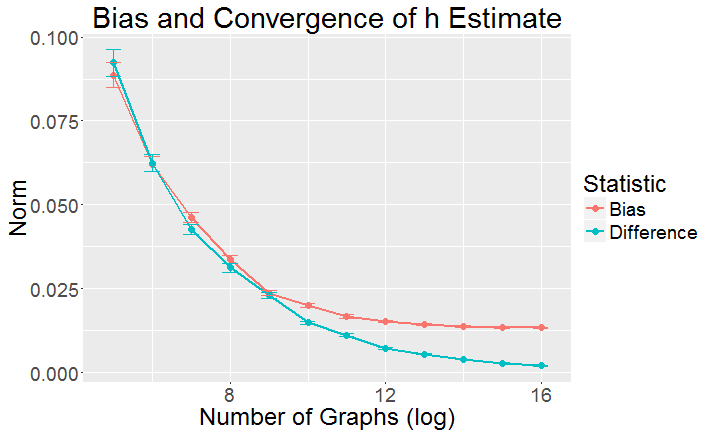
\includegraphics[scale=0.6,width=3.0in]{biasandconv.png}
	\caption{Bias and Convergence of Joint Embedding}
	%\label{fig:awesome_image}
\end{figure}

\noindent From the plot, we can see that  $||\hat{h}_1^m-\hat{h}_1^{\frac{m}{2}}||$ converges to $0$ as $m$ increases. It suggests the convergence of $\hat{h}_1^m$. Secondly, we should notice that the bias $||\hat{h}^m_1-h_1||$ does not converge to $0$; instead, it stops to decrease at around $0.03$. This suggests that $\hat{h}_1$ is an biased and asymptotically inconsistent estimator for $h_1$. The $\hat{h}_1^m$ with $m=2^{16}$ is $[0.083,0.186, 0.296, 0.406, 0.503]^T/0.74$. Compared to $h_1$, there are negative biases for small entries of $h_1$, and positive biases for large entries of $h_1$. Actually, there are some theoretical evidences for this phenomenon as well. In general, when there are infinitely many parameters present, in our case $\lambda_i$, we do not expect the unbiasedness of our estimators. \\

\noindent In applications like clustering or classifying graphs, we may not care about $\hat{h}_1$ at all. We are more interested in $\hat{\lambda}_i$ which specifically provides information about graph $i$. The bottom two plots are boxplots of $\hat{\lambda}_i$ for different values of $m$. The first one plots $\hat{\lambda}_i$ computed from joint embedding. The second one plots $\hat{\lambda}_i$ computed by forcing $\hat{h}_1$ equal to $h_1$. $\hat{\lambda}_i$ calculated this way can be thought of as 'oracle' estimates, since it assumes $h_1$ is known. Not surprisingly, the two plots look very similar since $||\hat{h}_1-h_1||$ is small for large $m$.
\begin{figure}[!htbp]
	\centering
	\includegraphics[scale=0.6,width=3.0in]{lambdahat.png}
	\caption{Boxplot for Lambda Estimates}
	%\label{fig:awesome_image}
\end{figure}
\begin{figure}[!htbp]
	\centering
	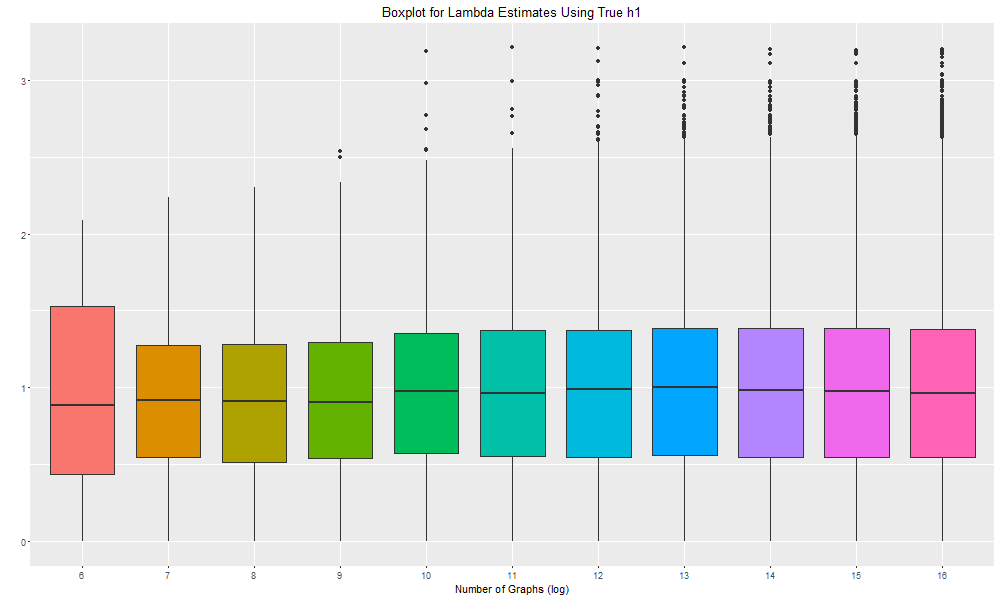
\includegraphics[scale=0.6,width=3.0in]{tlambdahat.png}
	\caption{Boxplot for Lambda Estimates Using True $h_1$}
	%\label{fig:awesome_image}
\end{figure}

\subsection{Simulation Experiment 2: Joint Embedding to Classify Graphs}
In this experiment, we consider the inference task of classifying graphs.  In general, $m$ pairs $\{(A_i,Y_i)\}_{i=1}^{m}$ are observed. Each pair consists of an adjacency matrix $A_i \in \{0,1\}^{n \times n}$ and a label $Y_i \in [K]$. Furthermore, all pairs are assumed to be independent and identically distributed according to an unknown distribution $\mathbb{F}_{A,Y}$, that is
\[(A_1,Y_1),(A_2,Y_2),...,(A_m,Y_m) \overset{i.i.d.}{\sim} \mathbb{F}_{A,Y} \] 
Our goal is to find a classification function $g:\{0,1\}^{n \times n} \rightarrow [K]$ which has small classification error $L_g=P(g(A)\neq Y)$. \\ 

\noindent Our experiment is set up to be a binary classification problem where $Y$ can only take value $0$ or $1$. We independently generate $200$ graphs with 100 vertices from two MREG models each. Let $h_1$ and $h_2$ be two vectors in $\mathbb{R}^{100}$, and \[h_1=[\frac{1}{10},\frac{1}{10},...,\frac{1}{10}]^T \text{ , and } h_2=[-\frac{1}{10},-\frac{1}{10},...,\frac{1}{10}]^T \] 
Here, $h_2$ has $-\frac{1}{10}$ as its first 50 entries and $\frac{1}{10}$ as its last 50 entries. Condition on the value of $Y$, we generate graphs according to two MREG models, that is 
\[A_i|Y_i=0 \sim MREG(F_0,h_1,h_2) \text{ , here } F_0= \mathbbm{1}_{[25,5]} \]
\[A_i|Y_i=1 \sim MREG(F_1,h_1,h_2) \text{ , here } F_1= \mathbbm{1}_{[22.5,2.5]} \]
In terms of SBM, this graph generation scheme is also equivalent to,
\[ A_i|Y_i=0 \sim  SBM((1,...,1,2,...,2),\begin{bmatrix} 0.3 & 0.2 \\ 0.2 & 0.3 \\ \end{bmatrix})  \]
\[ A_i|Y_i=1 \sim  SBM((1,...,1,2,...,2),\begin{bmatrix} 0.25 & 0.2 \\ 0.2 & 0.25 \\ \end{bmatrix})\]

\noindent To classify graphs, we first apply joint embedding algorithm to $200$ graphs. Then, a k-nearest neighbor classifier is constructed based on loadings $\hat{\Lambda}$ by treating ith row as a feature vector for graph $i$. The embeddings of $200$ graphs are shown in the figure below. We can see two classes are clearly separated after being jointly embedded. The 3-NN classification error is $0$. 

\begin{figure}[!htbp]
	\centering
	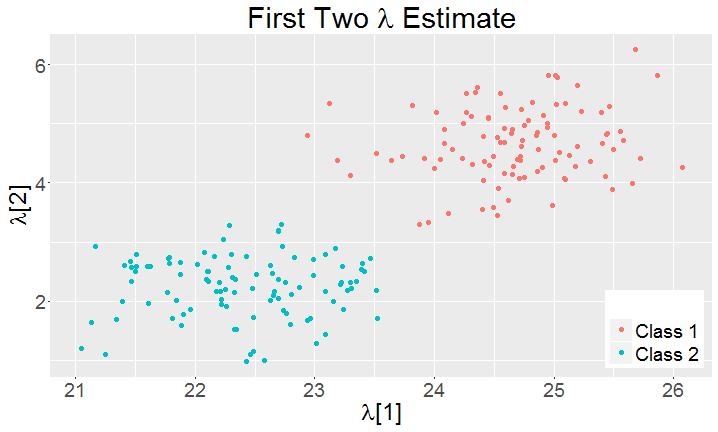
\includegraphics[scale=0.6,width=3.0in]{JE_200.png}
	\caption{$\Lambda_i$ of jointly embedded graphs}
	%\label{fig:awesome_image}
\end{figure}

\begin{comment}
\begin{enumerate}	
	\item We perform ASE on individual adjacency matrix $A_i$.
	\item We perform ASE on the average adjacency matrix $\bar{A}$, and use it as a latent position estimates for all graphs.
%	\item We jointly embed graphs ${A_i}_{i=1}^{m}$, and use $H |\Lambda_i|^{\frac{1}{2}}$ as latent position estimates for graph $i$.
	\item We first jointly embed graphs $\{A_i\}_{i=1}^{m}$, and cluster $\Lambda_i$ into clusters. Then we compute ASE on cluster conditional average adjacency matrix.
\end{enumerate}
To compare 3 approaches, we independently generate $100$ 100-vertex graphs from two stochastic block models each. Specifically,
\[ \{G_i\}_{i=1}^{100} \sim  SBM((1,...,1,2...,2),\begin{bmatrix} 0.3 & 0.2 \\ 0.2 & 0.3 \\ \end{bmatrix}) \text{ , and } \]
\[ \{G_i\}_{i=101}^{200} \sim  SBM((1,...,1,2...,2),\begin{bmatrix} 0.25 & 0.2 \\ 0.2 & 0.25 \\ \end{bmatrix})\]
The latent positions of class 1 graph is $(-0.50, -0.22 )$ and $(-0.50, 0.22 )$ for vertices in block 1 and 2 respectively. The latent positions of class 2 graph is $(-0.47, -0.16 )$ and $(-0.47, 0.16)$ for vertices in block 1 and 2 respectively. We fix the dimension of embeddings to be $2$ which allows us to compute Euclidean distance between latent position estimates and true latent positions. The $\Lambda$ of joint embeddings are displayed in the figure below. From it, we can clearly identify two clusters. The sum of estimation errors $\sum ||X_i-\hat{X}_i||$ is summarized in the following tables. We can see that approach 3 achieves the best latent position estimates.
\begin{center}
	\begin{tabular}{ | l | l | l|l| }
		\hline
		Approach & 1 & 2 &3  \\ \hline
		Error  & 705.92 & 77.56 & 49.96  \\ \hline 
	\end{tabular}
\end{center}

\end{comment}





\subsection{Real Data Experiment: CCI}








% references section

% can use a bibliography generated by BibTeX as a .bbl file
% BibTeX documentation can be easily obtained at:
% http://mirror.ctan.org/biblio/bibtex/contrib/doc/
% The IEEEtran BibTeX style support page is at:
% http://www.michaelshell.org/tex/ieeetran/bibtex/
%\bibliographystyle{IEEEtran}
% argument is your BibTeX string definitions and bibliography database(s)
%\bibliography{IEEEabrv,../bib/paper}
%
% <OR> manually copy in the resultant .bbl file
% set second argument of \begin to the number of references
% (used to reserve space for the reference number labels box)
\begin{thebibliography}{1}

\bibitem{IEEEhowto:kopka}
%H.~Kopka and P.~W. Daly, \emph{A Guide to \LaTeX}, 3rd~ed.\hskip 1em plus
%  0.5em minus 0.4em\relax Harlow, England: Addison-Wesley, 1999.

\end{thebibliography}

% biography section
% 
% If you have an EPS/PDF photo (graphicx package needed) extra braces are
% needed around the contents of the optional argument to biography to prevent
% the LaTeX parser from getting confused when it sees the complicated
% \includegraphics command within an optional argument. (You could create
% your own custom macro containing the \includegraphics command to make things
% simpler here.)
%\begin{IEEEbiography}[{\includegraphics[width=1in,height=1.25in,clip,keepaspectratio]{mshell}}]{Michael Shell}
% or if you just want to reserve a space for a photo:

%\begin{IEEEbiography}{Shangsi Wang}
%Biography text here.
%\end{IEEEbiography}

% if you will not have a photo at all:
%\begin{IEEEbiographynophoto}{Carey Priebe}
%Biography text here.
%\end{IEEEbiographynophoto}

% insert where needed to balance the two columns on the last page with
% biographies
%\newpage




\end{document}


